\chapter{Audioausgabe}
\label{Audioausgabe}
% ================ Einstellungen =======================
\thispagestyle{fancy} \rhead{\slshape Audioausgabe} 
% ======================================================
In diesem Kapitel werden die technischen Grundlagen welche sich auf das verwendete Audio-Modul beziehen, das Konzept sowie die Funktion der Audioausgabe beschrieben. Zudem wird die Validierung erläutert.
\section{Technische Grundlagen}
Für den Prototyp des Dojo’s wurde unter anderem ein WTV020 Chip verwendet. Das WTV020 Modul wird in diesem Kapitel beschrieben, da diese Informationen für die nachfolgenden Kapitel benötigt werden.\\
Das WTV020 Modul ist ein Soundmodul welches es ermöglicht Audiodateien auf einem Aktor abzuspielen. Auf einer maximal 1GB grossen $\mu$SD-Karte können bis zu 512 Audiodateien abgespeichert werden. Die Audiodateien auf der $\mu$SD-Karte müssen jedoch dem .wav oder.ad4 Format entsprechen. Die Dateien müssen gemäss Vorgabe: 0000; 0001; 0002; … nummeriert werden.\\
Der WTV020 Chip kann in zwei verschiedenen Modes betrieben werden, dem MP3 Mode und dem Two Line Serial Mode. Im MP3 Mode können direkt 6 Pins angesteuert werden. Durch die sechs Pins können folgende Funktionen umgesetzt werden: Reset, $\pm$Volume , next, previous und play, pause. 
Für das Dojo wird jedoch der two line serial mode genützt. Dieser kann das Modul mit nur 3 Pins betreiben. Der Mikrocontroller muss an den Clock-, den Data- und den Busy-Pin angeschlossen werden. Im two line serial mode können die Audiodateien welche sich auf der $\mu$SD-Karte befinden abgespielt werden. Er ermöglicht zudem, ähnlich wie im MP3 Mode ein Lied zu pausieren und neu zu starten, sowie eine Lautstärkenregulation.
\section{Konzept}
Das Konzept der Audioausgabe ist wie folgt aufgebaut:
\begin{figure}[h]
	\centering
	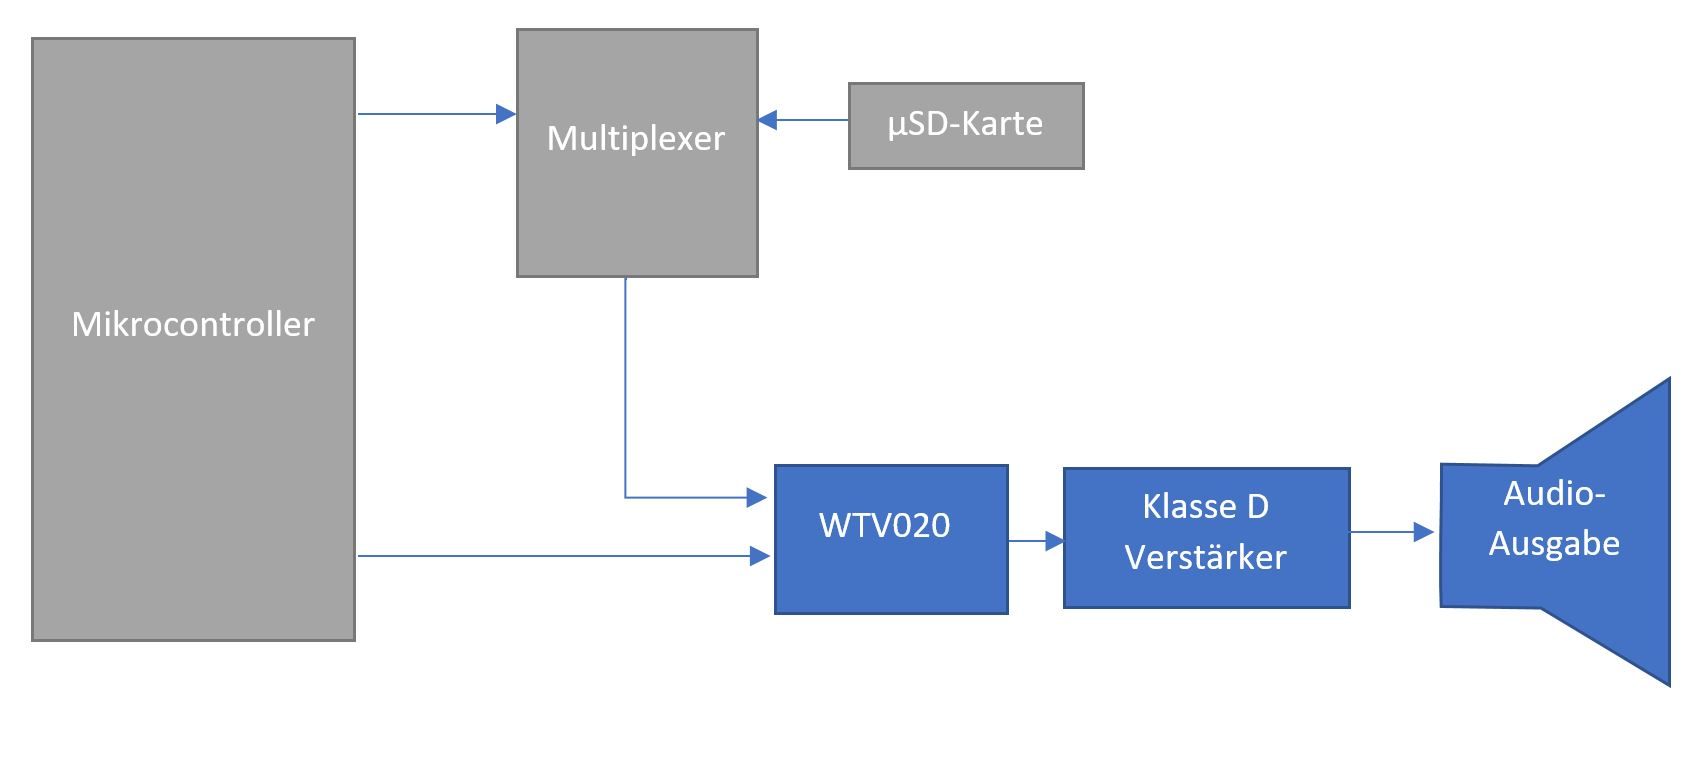
\includegraphics[width=15cm]{Bilder/Audio-Konzept.jpg}
	\caption{Audio Konzept}
	\label{Audio-Konzept}
\end{figure}
Die auf einer $\mu$SD-Karte abgespeicherten Audiodateien werden über einen Multiplexer, welcher vom Mikrocontroller gesteuert wird, an einen WTV020 Chip übertragen. Dieser wird in einem Serial Mode [Kapitel WTv020] betrieben und kann ebenfalls vom Mikrocontroller angesteuert werden. Der Audiochip entschlüsselt die Daten und gibt diese an einen Klasse D Verstärker weiter. Dieser wird benötigt um eine gut hörbare Lautstärke zu erreichen. Das Audiosignal wird schliesslich an einem Bone Conductor ausgegeben. 
Nachfolgend wird die Anordnung auf dem Print der einzelnen Komponenten dargelegt. 
\section{Hardware}
Wie im Konzept beschrieben, muss man, um Daten von der $\mu$SD-Karte auszulesen zuerst den Multiplexer ansteuern. Dies geschieht über den Mikrocontroller. Im ungesteuerten Zustand ist der MUX auf den VUB300 geschaltet. Sobald der MUX entsprechend angesteuert wird schalten die benötigten Kontakte. Der WTV020SD-20S Chip kann nun auf die $\mu$SD-Karte zugreifen. Über vier Pins werden die Audiofiles ausgelesen und weitergegeben. Das Audiosignal wird auf den Klasse-D Verstärker gegeben. Dieser ist wie folgt aufgebaut.
\begin{figure}[h]
	\centering
	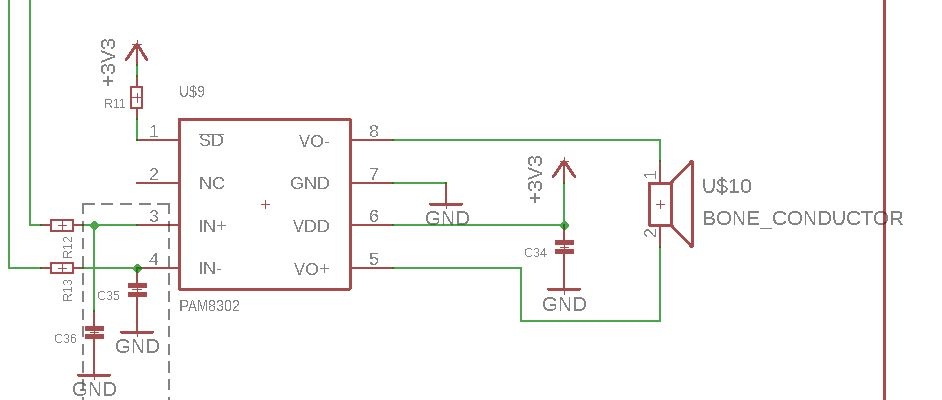
\includegraphics[width=15cm]{Bilder/Klasse-D.jpg}
	\caption{Klasse D Verstärker}
	\label{Klasse-D}
\end{figure}
Um ein Rauschen an der Speisung zu vermeiden wird ein ein$\mu$ Farad grosser Kondensator benötigt. In diesem Projekt wurde eine konstante Verstärkung mit dem Faktor ca.15 verwendet, da die Lautstärken Regelung über den WTV020-Chip geregelt werden soll. Dieser Faktor entsteht aus dem Verhältnis der Widerstände. Um das Rauschen der Eingänge sowie zu hohe Frequenzen zu filtern wurden zuerst wie die Abbildung \ref{Klasse-D} zeigt, Kapazitäten eingeplant. Auf dem Prototyp wurden aufgrund von Tests welche in der Validierung aufgeführt werden, die Kapazitäten weggelassen.\\ Wie erwähnt wird die Lautstärkenregelung über den WTV020-Chip geregelt. Dies ist jedoch im serial mode fehleranfällig. Aufgrund dessen wurde für die Tests ein 50 Ohm grosser Widerstand vor den Bone Conductor geschaltet da bei grossen Strömen dieser eine zu kleine Innenimpedanz aufweist.\\ Wie erwähnt wird die Lautstärkenregelung über den WTV020-Chip geregelt. Dies ist jedoch im serial mode fehleranfällig. Aufgrund dessen wurde für die Tests ein 50 Ohm grosser Widerstand vor den Bone Conductor geschaltet da bei grossen Strömen dieser eine zu kleine Innenimpedanz aufweist. Die Audioausgabe erfolgt wie beschrieben über einen Bone Conductor. Der Bone Conductor besteht aus einem kleinen Metallstab welcher mit einer Kupfer Spule umwickelt ist. Sobald ein pulsförmiger Strom durch die Spule fliest, dehnt sich ein Magnetfeld aus welches ein zusammenziehen auslöst. Der Bone Conductor ermöglicht es durch die Vibrationen das eine Audio Datei über den Schädelknochen abgespielt wird und so nur für eine Person hörbar ist, diese jedoch immer noch die Umgebungsgeräusche war nimmt.

\section{Firmware}
Wie im Kapitel Hardware beschrieben muss der MUX angesteuert werden um dem WTV-Chip den Zugriff auf die $\mu$SD-Karte zu gewähren. Die folgende Tabelle zeigt wie der MUX angesteuert werden muss, damit die benötigten Pins durgeschalten sind.

\begin{figure}[h]
	\centering
	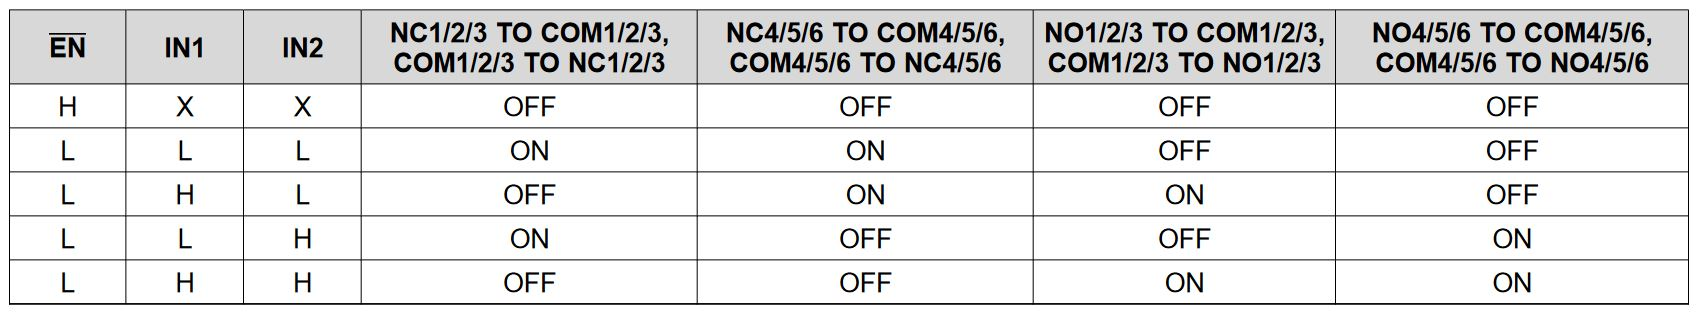
\includegraphics[width=15cm]{Bilder/MuxTab.jpg}
	\caption{MUX, TS3A27518 Funktionstabelle}
	\label{MUX-Tabelle}
\end{figure}

Für die Audioausgabe müssen alle Öffner geschlossen werden. Dies wird über die Pins 25 – 27 (Port C) realisiert. Sobald Musik abgespielt werden muss, werden die benötigten Ausgänge gesetzt. Sobald am Pin 9 über einen Taster Play ein low Signal erkannt wird, wird folgende Funktion aufgerufen:
\begin{figure}[h]
	\begin{verbatim}
void sendWTVcommand(unsigned int command){
	digitalWrite(WTV_CLK, LOW);
	_delay_us(1900);
	for (byte i = 0; i < 16; i++)
	{
		_delay_us(100);
		digitalWrite(WTV_CLK, LOW);
		digitalWrite(WTV_DOUT, LOW);
		if ((command & 0x8000) != 0)
		{
			digitalWrite(WTV_DOUT, HIGH);
		}
		_delay_us(100);
		digitalWrite(WTV_CLK, HIGH);
		command = command<<1;
	}
}
	\end{verbatim}
	\caption{Audio Datei abspielen }
	\label{WTV-Play}
\end{figure}


Die benötigten Befehle welche sendWTVcommand mitgegeben werden müssen sind aufgrund des WTV020-Chips vorgefertigt.
\newpage Nachfolgend werden die verwendeten Befehle aufgeführt.\\
OPCODEPLAYPAUSE: OPCODEPLAYPAUSE muss default mässig auf 0xFFE gesetzt werden. Dies ermöglicht es eine Datei abzuspielen und zu pausieren. Um die Ausgabe zu starten muss immer am Anfang die gewünschte File Nummer mitgegeben werden (0-512). Ohne File Nummer wird die Audioausgabe pausiert und kann wieder gestartet werden.  \\
OPCODESTOP: Dies stoppt die laufende Datei und setzt diese zurück.\\
OPCODEVOL: OPCODEVOL muss am Anfang auf 0xFFF0 gesetzt werden. Dies ermöglicht die Lautstärken Regulierung wobei 0xFFF0 den Aktor auf stumm schaltet und 0xFFF7 die maximale Lautstärke ausgibt. \\
Für die Audioausgabe wurden PLAYPAUSE und OPCODEVOL verwendet. Durch diese ist es möglich die gewünschten Funktionen umzusetzen. 

\section{Validierung}
Um die Audioausgabe zu testen, wurden verschiedene Versuche durchgeführt. Zuerst wurde der Bone Conductor über eine kleine Verstärkerschaltung direkt an einem Laptop angeschlossen, um die benötigte Leistung und die Lautstärke abschätzen zu können. Bei diesen Messungen ergab sich, bei einer sehr gut hörbaren Lautstärke, eine maximale Scheinleistung von 0.28 VA.\\
Da das WTV020 kleine Eigenheiten besitzt musste das Versuchsboard in dem im Kapitel (WTV tech Grundlagen) beschriebenen MP3 Mode betrieben werden. So konnten nicht kompatible $\mu$SD-Karten aussortiert werden. \\
Alle Funktionen des WTV020-Chips wurden separat überprüft. Alle verlangten Funktionen des Chips laufen wunschgemäss. Zudem wurde ein Versuchsaufbau mit dem D-Klasse Verstärker durchgeführt, mit welchem die aktuell maximal benötigte Leistung von XXXW gemessen wurde. \\
Trotz der funktionierenden Tests ist aktuell am Prototyp die Lautstärkenregelung nicht möglich. Das Audiomodul übernimmt die eingestellte Lautstärke, setzt diese jedoch meist wieder auf den vorherigen Wert. Zudem ist zu erwähnen, dass für eine Massenproduktion ein WTV020 Modul nicht geeignet wäre, aufgrund der erwähnten Eigenheiten. Das Modul nimmt trotz gleicher Formatierung und gleichem Hersteller nicht jede $\mu$SD-Karten an. Zudem treten beim serial mode immer wieder kleiner Ungereimtheiten auf, wie z.B. die Lautstärkenregelung. 
